%%%%%%%%%%%%%%%%%%%%%%%%%%%%%%%%%%
% EL Advance Electronic Engineering Report
% University of Southampton
%
% author : Lawrence Gray (lg5g15)
%
% edited : 2016-11-14
%%%%%%%%%%%%%%%%%%%%%%%%%%%%%%%%%%

\documentclass[a4paper,11pt]{article}
\setlength\parindent{0pt}
%%%%%%%%%%%%%%%%%%%%%%%%%%%%%%%%%%
% PACKAGES
%%%%%%%%%%%%%%%%%%%%%%%%%%%%%%%%%%
\usepackage[margin=1in]{geometry}
\usepackage{listings}
\usepackage{color}
\usepackage{float}
\usepackage{graphicx}
\usepackage[margin=2mm]{caption}
\usepackage{subcaption}
\usepackage{placeins}
\usepackage{amsmath}
\usepackage[english]{babel}
\usepackage[utf8]{inputenc}
\usepackage{url}
\usepackage{amsmath}
\usepackage{ulem}
\usepackage{enumerate}
\usepackage{amssymb}
%%%%%%%%%%%%%%%%%%%%%%%%%%%%%%%%%%
% DOCUMENT BEGIN
%%%%%%%%%%%%%%%%%%%%%%%%%%%%%%%%%

\begin{document}
  
\begin{center}

{\Large{\textbf{Digital Control ELEC3206:}}} \\ 
{\Large{\textbf{Lecture notes by Lawrence Gray}}} \\ [\baselineskip]
\end{center}
\section{Lecture 1: Intro }
	This course concerns using digital control using impulse sampling. The data is sampled using a train of impulses, in this example $x(t)$ is being sampled:
\begin{equation}
	x^*(t):= \sum\limits_{k=0}^{\infty}x(kT)\delta(t-kT)
	\end{equation}
	\subsection{Laplace to Z-Transform}
		The Laplacian transformation of a function $f(t)$ is:\\
		\begin{equation}
		\mathcal{L}(f):= \int\limits_{0}^{\infty}e^{-st}dt
		\end{equation}

		Example:\\
		
		\[ f(x) =\begin{cases} 
      			0 & t < 0\\
      			e^{\alpha t}& t \geq 0
   			\end{cases}
			\]

		\begin{equation}
		\mathcal{L}(f(t)):= \int\limits_{0}^{\infty}e^{\alpha t}e^{-st}dt =\int\limits_{0}^{\infty}e^{(\alpha -s)t}dt= \frac{1}{s-\alpha}		\end{equation}
		Below are some examples using the impulse response which is used a lot in this course:
		\begin{equation}
		    \mathcal{L}(\delta(\cdot))=1
		    \qquad
		    \mathcal{L}(\delta(\cdot-\tau))=e^{-s \tau}
		\end{equation}
		We can then simplify this further than laplace as we will always will be using a impulse.
		\begin{equation}
		    X^*(s)=\sum\limits_{k=0}^{\infty} x(kT)\mathcal{L}(\delta(\cdot-kT)) = \sum\limits_{k=0}^{\infty}x(kT)e^{-skT}= \sum\limits_{k=0}^{\infty}x(kT)z^{-k}
		\end{equation}
		We have defined z as:
		\begin{equation}
		    z=e^{sT}
		\end{equation}
		This brings the following definition of the Z transform:
		\begin{equation}
		    X(z):= \sum\limits_{\infty}^{k=0}x(kT)z^{-k}	
		\end{equation}		
\newpage
	\subsection{Z-transform of a sequence}
	For a sequence $\{x(kT)\}_{k=0,1...}$ we can find the Z transform of some common sequences:\\
	Sequence 1 is a impulse at 0 (Discrete Impulse):
	
		\[ x(kT) =\begin{cases} 
      			0 & k < 0\\
      			1 & k = 0\\
			0 & k > 0   			
   			\end{cases}
			\]
		Z-transform:
		\begin{equation}
		    X(z)= \sum\limits_{\infty}^{k=0}x(kT)z^{-k}=1\cdot z^{-0} = 1
		\end{equation}
	Sequence 2:
			\[ x(kT) =\begin{cases} 
      			0 & k < 0\\
      			1 & k = 0,1\\
			0 & k > 1   			
   			\end{cases}
			\]
		Z-transform:
		\begin{equation}
		    X(z)= \sum\limits_{\infty}^{k=0}x(kT)z^{-k}=1\cdot z^{-0} +1\cdot z^{-1}= 1+\frac{1}{z} = \frac{z+1}{z}
		\end{equation}
	Sequence 3:
			\[ e^{\alpha \cdot}  =\begin{cases} 
      			0 & t < 0\\
      			e^{\alpha t} & t \geq 0			
   			\end{cases}
			\]
		The laplace transform of this is given to be:
		\begin{equation}
		   \mathcal{L}(e^{\alpha \cdot})= \frac{1}{s-\alpha}
		\end{equation}
		To get the z transform of this we ``sample'' the signal  by stating $t=kT$ which makes our input function $e^{\alpha kT}$.\\
		So what is the Z-transform of $\{(e^{\alpha T})^{k}\}_{k=0,1...}$
		\begin{equation}
		    X(z)= \sum\limits_{\infty}^{k=0}(e^{\alpha T})^{k}z^{-k}=\sum\limits_{\infty}^{k=0}(\frac{e^{\alpha T}}{z})^{k}
		\end{equation}
		Here we assume that z is such that $|\frac{e^{\alpha T}}{z}|<1$. This then means that we can simply use the geometric series.
		\begin{equation}
		    X(z)= \sum\limits_{\infty}^{k=0}(\frac{e^{\alpha T}}{z})^{k}=\frac{1}{1-\frac{e^{\alpha T}}{z}}=\frac{z}{z-e^{\alpha T}}
		\end{equation}
	\subsection{Z-Transform rules}
		With a Z transform we convert a set of series of real numbers to a set of formal power series.
	Some Simple rules of the Z-transform (same as laplace I think):
		\begin{equation}
		    \mathcal{Z}(\{x_{k}+y_{k}\}) = \mathcal{Z}(\{x_{k})+\mathcal{Z}(y_{k}\})
		\end{equation}
		\begin{equation}
		    \mathcal{Z}(\{\alpha x_{k}\}) = \alpha\mathcal{Z}(\{x_{k}\})
		\end{equation}
	The Left Shift rule, here we are deriving the the Z-transform of $\mathcal{Z}(x_{k+1})$ we use a simple table to do so:
	

	\begin{center}
	\begin{tabular}{ |c|c|c|c|c| } 
	 \hline
	 k & 0 & 1 &2&3\\ 
	 \hline
	 $\{x_{k}\}$& $x_{0}$ & $x_{1}$& $x_{2}$& $x_{3}$\\ 
	\hline	 
	 $\{x_{k+1}\}$& $x_{1}$& $x_{2}$& $x_{3}$& $x_{4}$\\ 
	 \hline
	\end{tabular}
	\end{center}
	\begin{equation}
		X(z):= \sum\limits_{\infty}^{k=0}x_{k+1}z^{-k}=	x_{1} + x_{2}z^{-1} +x_{3}z^{-2}...= z\mathcal{Z}(\{x_k\})-zx_0
	\end{equation}
\section{Lecture 2:}
	Right Shift Rule $\{x(k-1)\}$ is simpler than the left shift rule:
	\begin{equation}
		\mathcal{Z}(\{x(k-1)\})=z^{-1}\mathcal{Z}(\{x(k)\})
	\end{equation}
	Convolution, $\{h(k)\}:=\{x(k)\}*\{y(k)\}$, is also a simple rule:
	\begin{equation}
		h(k) = \sum\limits_{k}^{j=0}y_{k-j}x_j
	\end{equation}
	\begin{equation}
		\mathcal{Z}(\{h(k)\})=\mathcal{Z}(\{x(k)\})\mathcal{Z}(\{y(k)\})
	\end{equation}\\
	Initial Value theorem, for our initial value $x_0$:
	\begin{equation}
		\mathcal{Z}(\{x(k)\})=x_0+x_1x^{-1}...
	\end{equation}
	From this we can then find the initial value as z tends to $\infty$ 
	\begin{equation}
		x_0=\lim\limits_{z \rightarrow \infty}\mathcal{Z}(\{x_k\})
	\end{equation}
	\subsection {Final Value Theorem:}
		if $\mathcal{Z}(\{x_k\})$ has all of it's singularities in the open unit circle except possibly in the open unit circle except possibly one at $z=1$ then $\lim\limits_{Z\Rightarrow\infty}(x_k)=\lim\limits_{z\Rightarrow\infty}(1-z^{-1})\mathcal{Z}(\{x_k\})$.\\
		Note, for this course, almost all Z-transforms are rational functions so ``singularity" means 0 at the denominator/``pole"
	\subsection{Fibonacci sequence/Difference equation}
		A Fibonacci sequence is defined as:
		\begin{equation}
		    y(k+2)=y(k+1)+y(k)
		\end{equation}
		But in digital control we tend to see this with an extra term which we think of as our input:
		\begin{equation}
		    y(k+2)-y(k+1)-y(k) = u(k)
		\end{equation}
		The main features of the difference equation are:
		\begin{itemize}
		    \item Order = highest shift - lowest shift
		    \item Linear
		    \item coefficients do not depend on time 
		\end{itemize}
		A real world example is a bank account, where $S(k)$ is the sum of money, $\alpha(k)$ is the interest rate and $u(k)$ represents deposits and withdrawals:
		\begin{equation} 
			S(k+1)= S(k) +\alpha(k)S(k) +u(k)
		\end{equation}
	\subsection{Difference equation in Signal processing}
		\begin{equation} 
			y(k+2)-y(k+1)-y(k)=u(k)
		\end{equation}	
		\begin{equation} 
			\mathcal{Z}(y(k+2))-\mathcal{Z}(y(k+1))-\mathcal{Z}(y(k))=\mathcal{Z}(u(k))
		\end{equation}
		We will derive the second shift to preform a Z-transform on the above equation.\\
		The second shift, $y(k+2)$ is the left shift of $y(k+1)$
		\begin{equation} 
			\mathcal{Z}(y(k+2))=z\mathcal{Z}(y(k+1))-zy_1=z(zY(z)-zy_0)-zy_1
		\end{equation}
		Now we can derive $Y(z)$:
		\begin{equation} 
			(z^2Y(z)-z^2y_0-zy_1)-(zY(z)-zy_0) -Y(z) = U(z)
		\end{equation}	
		\begin{equation} 
			(z^2-z-1)Y(z) = z^2y_0+zy_1-zy_0 +U(z)
		\end{equation}
		\begin{equation} 
			Y(z) =\frac{z^2y_0+zy_1-zy_0}{z^2-z-1}+\frac{1}{z^2-z-1}U(z)
		\end{equation}	\\
		FREE RESPONSE: The first expression on the right hand side is the Z-transform of the solution to the equation $y(k+2)-y(k+1)-y(k)=0$ with initial conditions $y_0$ and $y_1$. This is how the system acts if no external (force) is applied.\\\\
		FORCED RESPONSE: The second expression of the right hand side is the Z-transform of the solution to the equation $y(k+2)-y(k+1)-y(k)=0$ with initial conditions $y_0=y_1=0$ and the "forcing term" (input) being $u(k)$.\\
		$\mathcal{Z}("sequence")=Transfer Function$
\section{Lecture 3: Stability}
	Issue: how to characterise the system s that (for zero initial conditions) react reasonably to a reasonable input.\\
	We define reasonable as ``bounded". $\{u_k\}$ is bounded if there exists an $M$ such that $|u_k|<M $ for $k=0,1,...$\\
	A system is said to be stable if bounded inputs produce bounded outputs (for zero initial conditions).\\\\
	For this next section we will be considering the equation $Y(z)=H(z)U(z)$ where H(z) is the transfer function.\\
	$U(z)$ rational funtion: when is it the Z-transform of a bounded signal?\\
	for $U(k)=\{\alpha^k\} \rightarrow^\mathcal{Z} \frac{z}{z-\alpha}$ the condition $|\alpha|<1$(within unit circle) must hold true to be bounded.\\
	$Y(z)$ rational comes from a bounded sequence if and only if all of its poles are in an open unit disk ($\mathcal{D}$).\\
	From this, if $U(z)$ has all of its poles in $\mathcal{D}$ then $Y(z)$ has all its poles in $(\mathcal{D})$ of and only if $H(z)$ has all of its poles in the unit circle $\mathcal{D}$.\\\\
	Theory:
	\indent The system with TF $H(z)$ is bounded input bounded output stable (BIBO-stable) if and only if all the poles of $H(z)$ are in $\mathcal{D}$.\\
	Note the "open" unit dis is for $|z|<1$ not \sout{$|z|\leq1$}.\\
	Example of unbounded:
	\begin{equation}
		H(z) = \frac{z}{z-1} \qquad \{u_k\}=\{1,1,1,1...\}
	\end{equation}
	\begin{equation}
	    	Y(z) = H(z)U(z)=\frac{z}{z-1}\frac{z}{z+1}\Rightarrow\{0,1,2,3...\}
	\end{equation}
	Therefore this is unbounded.\\
	\subsection{Sampling}
		\textbf{DAC:(zero order hold)}\\
		The zero order hold keeps the sample constant between samples. 
		\begin{equation}
			U(t)=U_d(k)\qquad kT\leq t < (k+1)T		
		\end{equation}
		\textbf{Sample and Hold block model:}\\
		To understand this we will use a unit step input defined as:
		\[\bar{1}(t) =\begin{cases} 
      			1 & t \geq 0\\
      			0 & t < 0			
   			\end{cases}
			\]
			
		\begin{figure}[htp]
		\centering
		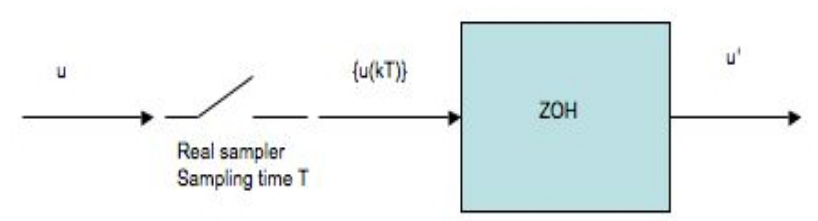
\includegraphics[scale=0.4]{images/sample_and_hold}
		\end{figure}
		\begin{equation}
			u'(t)=\sum\limits_{k=0}^{\infty}u(kT)[\bar(1)(t-kT)-\bar(1)(t-(k+1)T)]		
		\end{equation}
		As I cant be bothered to draw it i'm going to describe what this is doing. This part $[\bar(1)(t-kT)-\bar(1)(t-(k+1)T)]$ creates a unit pulse of length T between $kT$ and $(k+1)T$.\\
		We next take the laplace of that: 
		\begin{equation}
			\mathcal{L}(u')=\sum\limits_{k=0}^{\infty}u(kT)[\mathcal{L}(\bar(1)(t-kT))-\mathcal{L}(\bar(1)(t-(k+1)T))]
		\end{equation}	
		\begin{equation}
			=\sum\limits_{k=0}^{\infty}u(kT)[\frac{e^{-(k+1)Ts}}{s}-\frac{e^{-kTs}}{s}]=\sum\limits_{k=0}^{\infty}u(kT)[\frac{e^{-kTs}(1-e^{-Ts})}{s}]
		\end{equation}
		\begin{equation}
			\mathcal{L}(u')=\frac{1-e^{-Ts}}{s}U^*(s)
		\end{equation}	
		\subsection{Frequency response of ZOH}
		\begin{equation}
			G(s)=\frac{1-e^{-Ts}}{s}\rightarrow G(jw) = 1-e^{-Tjw}=2e^{-Tjw}\frac{e^{\frac{T}{2}jw}-e^{\frac{-T}{2}jw}}{2jw}
		\end{equation}
		\begin{equation}
			=\frac{T\sin(w\frac{T}{2})}{w^{\frac{T}{2}}}e^{-\frac{T}{2}jw}
		\end{equation}
		where $\frac{T\sin(w\frac{T}{2})}{w^{\frac{T}{2}}}$ is the sinc function.\\
		\FloatBarrier
		\begin{figure}[htp]
		\centering
		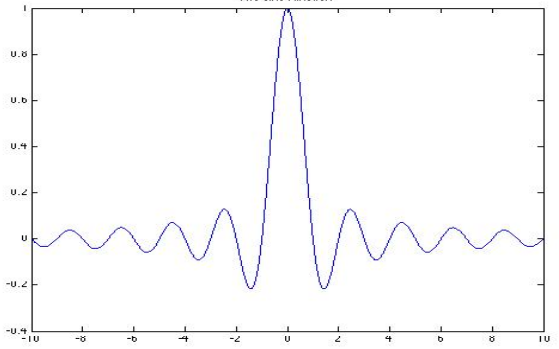
\includegraphics[scale=0.4]{images/sinc}
		\end{figure}
		
		I wrote this down but cannot remember the relevance any more.\\
		\begin{equation}
		    	(g*u)(t)=\int\limits_{-\infty}^{\infty}g(t-\tau)u(\tau)d\tau
\end{equation} 
\section{Lecture 4: Reconstruction of signals from samples}
\subsection{First Order Sample and hold}
	The for the input $u(t)$, sampled value of $\{u(kT)\}$ and the output $u'(t)$.
	The First order hold is defined as:
	\begin{equation}
		u'(t):= u_d(kT)\frac{t+T}{T}-u_d((k-1)T)\frac{t}{T} for kT \leq t < (k+1)T
	\end{equation}
	When we take $u_d$ as the step input ($\bar{1}$) we get:
	\begin{equation}
		u'(t)= \bar{1}(t)\frac{t+T}{T}-\bar{1}(t-T)\frac{t-T}{T}-\bar{1}(t-T) 
	\end{equation}
	Using the laplace and the shifting rules we obtain:
	\begin{equation}
		\mathcal{L}(u')= (\frac{1}{Ts^2}+\frac{1}{s})-e^{-Ts}\frac{1}{Ts^2}-e^{-Ts}\frac{1}{s1}= (1-e^{-Ts})\frac{Ts+1}{Ts^2}
	\end{equation}	

\subsection{Reconstruction of signals from samples}
	Shannon's sampling theorem:\\
	For a signal $f(.)$ which is band limited over the whole real axis, therefore $F(w)=0$ for $w<-w1$ and $w>w_1$.(This is basically just stating that that the maximum frequency is given as $w_1$).\\
	Shannon's theorem state that, if the sampling frequency $ w_s > 2 w_1$ then $f(.)$ can be uniquely reconstructed from its samples.\\
	Moreover...what is the significance of this?
	\begin{equation}
		f(t)=\sum\limits_{\infty}^{k=-\infty}f(kT)\frac{sin(\frac{w_s(t-kT)}{2})}{\frac{w_s(t-kT)}{2}}= \sum\limits_{\infty}^{k=-\infty}sinc(\frac{w_s(t-kT)}{2})
	\end{equation}
	
	Proof of this can be done using forrier series. Here is a quick definition of how to move from frequency domain to the time domain:
	\begin{equation}
		F(w)=\int\limits_{-\infty}^{\infty}e^{-jwt}f(t)dt
	    	\qquad
	    	f(t)=\frac{1}{2\pi}\int\limits_{-\infty}^{\infty}e^{jwt}F(w)dw
	\end{equation}	
	We then define the fourier transform of the sampled signal as:
	\begin{equation}
		F_s(w):=\frac{1}{T}\sum\limits_{k=-\infty}^{\infty}F(w+kw_s)
	\end{equation}	
	If $w_s>2w_1$:
				\[ F(w) =\begin{cases} 
      			TF_s(2) & |w|\leq \frac{w_s}{2}\\
      			0 & |w| >\frac{w_s}{2} 			
   			\end{cases}
			\]
	
	Fourier series of $F_s$ is: 
	\begin{equation}
	    F_s(w) = \sum\limits_{k=-\infty}^{\infty}C_ke^{-jwkT}
	\end{equation}
	where: 
	 \begin{equation}
	    C_k=\frac{1}{w_s} \int\limits_{0}^{\infty}e^{jwkT}F_s(w)dw
	\end{equation}
	
	
	Compute:
	 \begin{equation}
	    f(kT)=\frac{1}{2\pi}\int\limits_{-\infty}^{\infty}e^{jwkT}F(w)dw=\frac{1}{2\pi}\int\limits_{-\frac{w_s}{2}}^{\frac{w_s}{2}}e^{jwkT}TF_s(w)dw=\frac{1}{w_s}\int\limits_{-\frac{w_s}{2}}^{\frac{w_s}{2}}e^{jwkT}F(w)dw= C_k
	\end{equation}
		
	Apparently this shows that we can reconstruct $F_s(w)$.\\
	
	Causal definition: "A system is said to be causal system if its output depends on present and past inputs only and not on future inputs."\\
	The sinc function is not causal, even approximating it by truncation (waiting for more inputs before making decision), a delay is introduced. Not suitable for time critical applications in control.\\
	
	\subsection{Aliasing \& Folding}
	The forrier series of the sampled signal was previously given as:
	 \begin{equation}
		F_s(w):=\frac{1}{T}\sum\limits_{k=-\infty}^{\infty}F(w+kw_s)
	\end{equation}
	Here you should consider what this is representing. Imagine $F(w)$ is the frequency response which will be centred around 0. Therefore the summation $F(w+kw_s)$ creates many copies of that given response. For $w_s>2w_1$ we can see that the spectra do not intersect (in this case then signal can be reconstructed).
	\FloatBarrier
	\begin{figure}[htp]
		\centering
		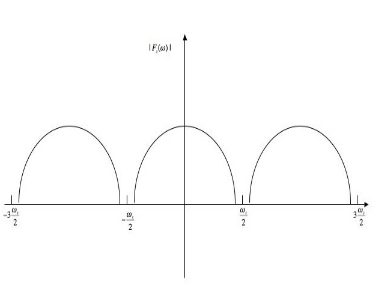
\includegraphics[scale=0.5]{images/aliasing_and_folding_1}
	\end{figure}
	But if we have $w_s\leq0$ then the spectra intersect. This is also known as the folding phenomenon. 
	
	\FloatBarrier
	\begin{figure}[htp]
		\centering
		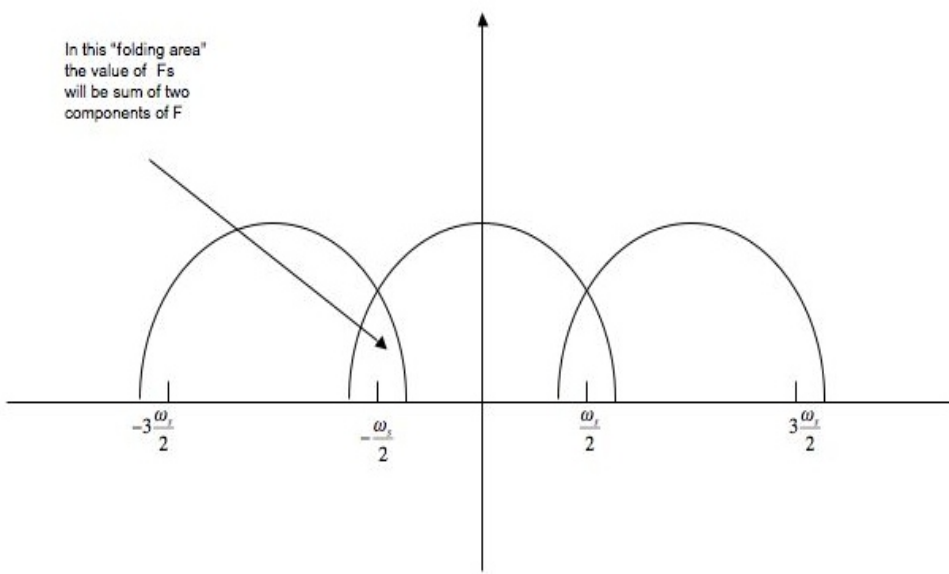
\includegraphics[scale=0.25]{images/aliasing_and_folding_2}
	\end{figure}
	Summary: 
	"If $\frac{w_s}{2}\leq$ then frequencies higher than appear “folded” between 0 and $\frac{w_s}{2}$. Sampling at frequencies lower than the Nyquist one $\frac{w_s}{2}$ can hide frequencies."
	\subsection{Example: Sinusoidal input to sample-and-hold}
	I would take this with a pinch of salt, the maths are all valid but i'm not sure what this achieves really.\\
	modulate $u(t)= sin(wt+\phi)=im(e^{j(wt+\phi)})$ with $\sum\limits_{k=-\infty}^{\infty}\delta(t-kT)$ which has the representation:
	\begin{equation}
		\sum\limits_{k=-\infty}^{\infty}e^{-kjw_st}= 2\sum\limits_{k=0}^{\infty}cos(kw_st)    
	\end{equation}
	Here is a quick proof of this as given in the lecture:
	\begin{equation}
		2\sum\limits_{k=0}^{\infty}cos(kw_st)= ...+e^{2jw_st}+e^{jw_st}1+1+e^{-jw_st}+ e^{-2jw_st}+...    
	\end{equation}
	Using the exponential definition of cos(t):
	\begin{equation}
		cos(t)= \frac{e^{jt}+e^{-jt}}{2} 
	\end{equation}
	You can then pair up the terms and see that the previous equation holds true.\\
	End of proof.\\\\
	
	The output of the sampler is:
	\begin{equation}
		\frac{1}{T}(\sin(wt+\phi)+2\sum\limits_{k=1}^{\infty}\cos(kw_st)\sin(wt+\phi) 
	\end{equation}
	which can be found to be equal to:
	\begin{equation}
		\frac{1}{T}(\sin(wt+\phi)+2\sum\limits_{k=1}^{\infty}\sin(kw_st+wt+\phi) -\sin(kw_st-wt-\phi))
	\end{equation}
	This finds that there are frequency components at $w\pm kw_s$:
	\FloatBarrier
	\begin{figure}[htp]
		\centering
		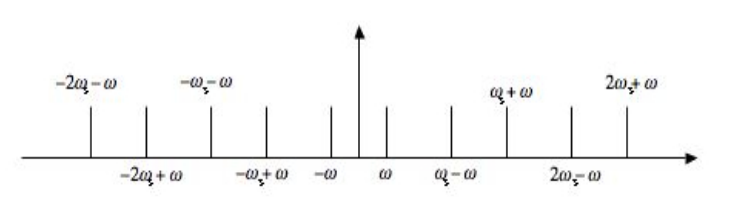
\includegraphics[scale=0.5]{images/sample_and_hold_freq}
	\end{figure}
	Through zero order hold block, for $w\neq\frac{w_s}{2}$, fundamental component at $w$ is transformed to:
	\begin{eqnarray}
		u_r(t)=\frac{1}{T}im(G(jw)e^{j(wt+\phi)})
	\end{eqnarray}
	But for $w=\frac{w_s}{2}$ this produces two components in the sampled signal. in this case the output after a zero order hold bloc:
	\begin{eqnarray}
		u_r(t)=\frac{1}{T}im(2e^{j(\pi -\phi)}sin(\phi)G(jw)e^{j(wt+\phi)})
	\end{eqnarray}
	Notice the dependence on $\phi$ as in this case if it is equal to $\pi$ then $u_r=0$.\\
	Sampling at or under the Nyquist rate for reconstruction the phase is crucial therefore you should never trust the reconstructed signal.\\
	
	In his slides he then gives graphical examples of this, but its quite self explanatory, if the samples occur whenever the signal is 0 then you have nothing to reconstruct!.
	
	
	\subsection{Choice of sampling period}
	\begin{itemize}   
		\item Choice of T related to physical, technological, cost, etc. factors
		\item Shannon's result = ideal situation: infinite accuracy, band limited signal, perfect reconstruction.
		\item In reality: quantization effect, unmodelled dynamics, disturbances, structure of controller, unknown highest frequency $w_1$, etc.
		\item Effect: spurious low frequencies due to folding and aliasing of high frequencies
		\item Rule of thumb: take frequency $2w_1$, and multiplyby 5 to 20 in order to find sampling frequency.
		\item Too high? Then decrease and check if controlled system still performs well.
		\item Or, use antialiasing filters (Bessel, Butterworth, etc.) to bandlimit signal before sampling in order to obtain reasonable sampling rate.
	\end{itemize}
	
	\subsection{Pre filtering} 
	This is quite self explanatory so i'm just going to copy from the slides.\\	To avoid aliasing problems, it may be useful to
prefilter the analog signals before sampling.\\
	Analog sensors have some filter integrated, but it is
not especially designed for your control problem!\\
Easier way out: introduce analogue filter (e.g. Bessel)
before the sampler. That will reduce the input signal
bandwidth, and guarantee that no aliasing appears.\\
If the analogue filter has non-negligible effects on the
dynamics of the control system, then it must be taken
into account in the control design.\\
	\section{Lecture 5: Pulse Transfer Functions} 
	\begin{figure}[htp]
		\centering
		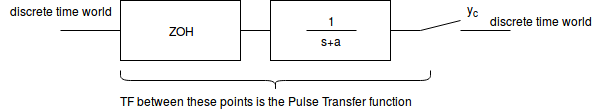
\includegraphics[scale=0.6]{images/PTF}
	\end{figure}
	\FloatBarrier
	
	``The transfer function is a faithful representation of the I/O behaviour of a linear system at rest."
	With the transfer function being $H(s)$: 
	\begin{equation}
		Y(s)=H(s)U(s)
	\end{equation}
	If I do not know $H(s)$, in principle I can recover it from experiments.
	\begin{equation}
		H(s):=\frac{Y(s)}{U(s)}
	\end{equation}
	The procedure to find the PTF is:
	\begin{enumerate}[a)]
		\item take $u(.)$ (discrete time) and take its Z-transform $U(z)$
		\item ZOH $u(.)$ and find $y(.)$ at continuous time at ($y_c$) 
		\item (Ideally) sample $y(.)$ and Z-transform the result by obtaining $Y(z)$
		\item Define PTF by $\frac{Y(z)}{U(z)}$
	\end{enumerate}
	In principle, ant $u(.)$(Discrete time) could do for the experiment but life is easier if $u_k=1$ for $k=0,1,...$\\
	The reason for this is that the ZOH reconstruction of a discrete time step is equivalent to a continuous time step.
	The relation between $y_c(.)$ and $u_c(.)$ is(in the laplace domain):
	\begin{equation}
		Y_c(s)=\frac{1}{s+\alpha}U_c(s)
	\end{equation}  
	Since ${u_k}={1,1,1...}$ $\rightarrow$ $\bar1(.)$(heaviside step) then $\mathcal{L}(u_c)=\frac{1}{s}$\\\\
	Therefore we can find:
	\begin{equation}
		Y_c(s)=\frac{1}{s+\alpha}\frac{1}{s}=\frac{-\frac{1}{\alpha}}		{s+\alpha}+\frac{\frac{1}{\alpha}}{s}
	\end{equation}
	\begin{equation}
		y_c = -\frac{1}{\alpha}(e^{-\alpha t})+\frac{1}{\alpha}\bar1(t) \qquad t\geq 0
	\end{equation}
	Sampling with sample period T and take Z transform:
	\begin{equation}
		\mathcal{Z}(y_k)=-\frac{1}{\alpha}\mathcal{Z}(e^{\alpha kT})+\frac{1}{\alpha}\mathcal{Z}(1)=-\frac{1}{\alpha}\frac{z}{z-e^{-\alpha T}}+\frac{1}{\alpha}\frac{z}{z-1}
	\end{equation}
	From this we can define $Y(z)$:
	\begin{equation}
		Y(z) := \frac{z(1-e^{1-\alpha T})}{\alpha (z-e^{-\alpha T})(z-1)}
	\end{equation}			
	We have already discussed the definition of $U(z)$:
	\begin{equation}
		U(z) := \mathcal{Z}(\{u_k\})=\frac{z}{z-1}
	\end{equation}	
	We can now get $H(z)$(PTF) from these two above equations:
	\begin{equation}
		H(z)=\frac{Y(z)}{U(z)}=\frac{1-e^{-\alpha T}}{\alpha(z-e^{-\alpha T})}
	\end{equation}
	He then drew a table kind collating the information obtained above but I don't want to draw that out now.\\
	In general we try to conciser an $\alpha$ value less than 0.\\
	
	\begin{figure}[htp]
		\centering
		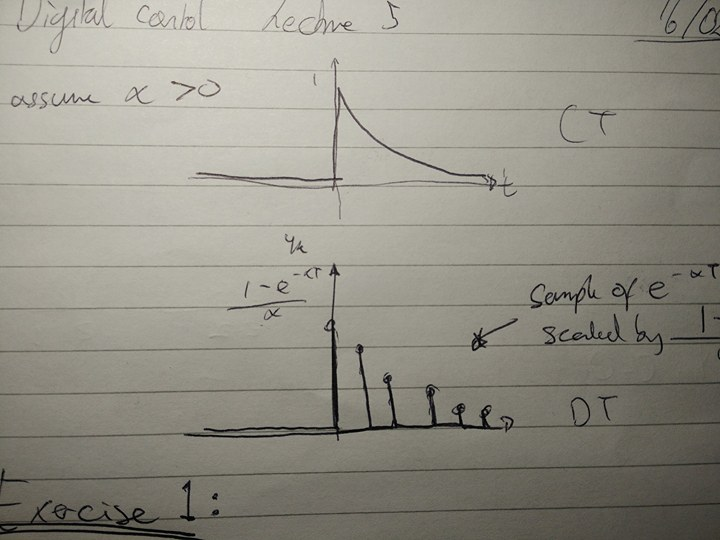
\includegraphics[scale=0.4]{images/CT-DT}
	\end{figure}
	Some general points about PFT:
	\begin{enumerate}[a)]
		\item Discretion via PFT involves scaling
		\item The PFT may have zeros even if the (CT)TF did not have any.
		\item A CT (stable/unstable) TF is made discrete into a DT (stable/unstable) TF (because poles in the LHP are transformed into/outside of the unit disk)\\
	\end{enumerate}
	A ``Zero" is by definition a root of the numerator of the TF, but we need to think about its dynamical interpretation. Lets consider:
	\begin{equation}
		H(z) = \frac{z-4}{(z-2)(z-3)}\qquad U(z)= \frac{z}{z-\alpha}\qquad Y(z)=\frac{z-4}{(z-2)(z-3)}\frac{z}{z-\alpha}
	\end{equation} 
	\begin{equation}
		=\frac{A}{z-2}+\frac{B}{z-3}+\frac{C}{z-\alpha}
	\end{equation} 
	when does $C=0$? If and only if $\alpha = 4$\\
	``Zeros represent frequencies which ``disappear" when provided as an input to the system"\\
	Mapping poles from s space to z space can be seen here:
	\FloatBarrier
	\begin{figure}[htp]
		\centering
		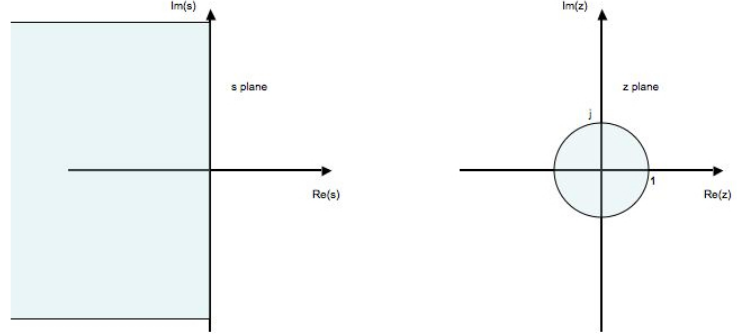
\includegraphics[scale=0.3]{images/mapping}
	\end{figure}
	\FloatBarrier
	
	note on cascaded element, in the below figure the top sequence is not equal to the bottom. 
	\FloatBarrier
	\begin{figure}[htp]
		\centering
		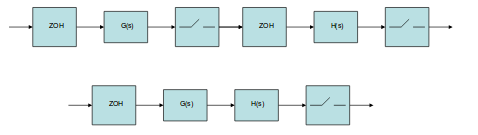
\includegraphics[scale=0.7]{images/cascading}
	\end{figure}
	\section{Lecture 6: State-Space Equations}
	In order to give an introduction to state space equations we will be giving an example of a simple one first.
	If we consider the population of a species at time k.\\
	$Y(k)$ is the number of young individuals at time k.\\
	$M(k)$ is the number of mature individuals at time k.\\
	$O(k)$ is the number of old individuals at time k.\\
	This then leads to a set of equations which determines these three things.\\	
	$O(k+1)=\alpha M(k)$ for $0 \leq \alpha \leq 1$ (you need to be mature before you can be old)\\
	$M(k+1)=\beta Y(k)$ for $0 \leq \alpha \leq 1$ (you need to be young before you can be mature)\\
	$Y(k+1)=\gamma M(k)$ for $0 \leq \alpha \leq 1$ (mature people give birth to kids)\\\
	we can then arrange this into matrix form:
	
\begin{gather}
x(K+1)=
 \begin{bmatrix} Y(k+1) \\ M(k+1 )\\ O(k+1)\end{bmatrix}
 =
  \begin{bmatrix}
	0 & \gamma & 0 \\
	\beta & 0 & 0 \\
	0 & \alpha & 0 
   \end{bmatrix}
    \begin{bmatrix} Y(k) \\ M(k)\\ O(k)\end{bmatrix}
    := A x(k)
\end{gather}

Using this we will consider a close population system ($x(0)$ is known), therefore we can start deriving the population at time k+1:\\
$k=0$ $x(1)=Ax(0)$\\
$k=1$ $Ax(1)=AAx(0)=A^2x(0)$ and so on...\\
which brings about the formula $x(k)=A^kx(0)$\\\\
Now we consider more complications in our model (Migration/Culling/Immigration):\\
To do this we consider $u(k)$ which is the number of population entering/exiting at time k.\\
\begin{gather}
 \begin{bmatrix} \eta \\ \delta \\ \epsilon\end{bmatrix}u(k)
\end{gather}
where $\eta$ is the number of young entering/exiting ... and so on. Also note $\eta+\delta+\epsilon = 1$. Adding this to our original equation gets us:
\begin{gather}
x(k+1)=
 \begin{bmatrix} Y(k+1) \\ M(k+1 )\\ O(k+1)\end{bmatrix}
 =
  \begin{bmatrix}
	0 & \gamma & 0 \\
	\beta & 0 & 0 \\
	0 & \alpha & 0 
   \end{bmatrix}
    \begin{bmatrix} Y(k) \\ M(k)\\ O(k)\end{bmatrix}
\end{gather}
We can also calculate the total populations using:
\begin{gather}
y(k)=
 \begin{bmatrix} 1\\ 1\\ 1\end{bmatrix}
	x(k)
\end{gather}

this leads the the following two equations:
\begin{equation}
	x(k+1) = A x(k) + Bu(k)
\end{equation}
\begin{equation}
	y(k) = C x(k) + Du(k)
\end{equation}

Some important information about these is that $x(k)$ has n components, $u(k)$ has m components and $y(k)$ has p components. Which leads to $A\in \mathbb{R}^{n\times n}$, $B\in \mathbb{R}^{n\times m}$, $C\in \mathbb{R}^{p\times n}$ and  $D\in \mathbb{R}^{p\times m}$.\\\\
Possible equations for the population model:
\begin{enumerate}[a)]
	\item Which policy (choice of $\eta$, $\delta$ and $\epsilon$) of culling/introduction guarantees that a specific distribution in young-mature-old is maintained? ``controllability"
	\item How to compute or determine distribution young-old-mature looking at $y(.)$? ``observability"
	\item Will the population die out or will it reach stable value or will it explode ? ``stability"
	\item Maximise a quadratic function of the state space equation and the input. ``optimal control"
\end{enumerate}

Solution to the state-space equation:\\
$x(0)$ given $x(k+1)= Ax(k)+Bu(k)$ where u(0), u(1)... is given.\\
For discrete time:
\begin{equation}
	x(k) = A^kx(0)+\sum\limits_{k-1}^{j=0}A^{k-1-j}u(j)    
\end{equation}
for continuous time:
\begin{equation}
	x(t) = e^{A\tau}+\int\limits_{0}^{t}e^{A(t-\tau)}Bu(\tau)d\tau    
\end{equation}
\section{Lecture 7 ( State-Space Self Study)}
This worksheet contains 2 methods of solving state-space equations, both in the time domain and the Z-domain. (basic idea: Z domain is easier than time domain). I will skip over the solution in the time domain for now as it seems this was just trying to prove a point.
\subsection{Z-Transform solution}
We will consider the state-space equation from the previous lecture. But first we will rewrite $y(k)$ in terms of $x(0)$:
\begin{equation}
    y(k) = CA^kx(0)+\sum\limits_{k-1}^{j=0}CA^{k-1-j}Bu(j) + Du(k)  
\end{equation}
Using Z-Transforms make sure you are happy deriving the following from the defintion of the $x(\cdot)$:
\begin{gather}
	zX(z) - zx(0) = \mathcal{Z}(Ax(.)+Bu(.))= AX(z)+BX(z)\\
	\qquad \rightarrow zX(z)-AX(z)=zx(0)+BU(z)\\
	\qquad \rightarrow (zI - A)X(z)= zx(0)+BU(z)
\end{gather}
From here it is quite simple. You can see that in order to find $X(z)$ you must find $(zI-A)^{-1}$ and then just simplify the right hand size. From this take the inverse transform to get x(k).
\subsection{The rest}
	There was a bit more to this lecture but as it was mainly an exercise it's kind of hard to write in note form. But here are some other noteable things that should be taken, mainly concerning matrix multiplication.\\\\
	A matrix $A$ can be written as a cobination of matricies. An example of this is $A=T\Lambda T^{-1}$ where $\Lambda$ is a diagonal matrix of eigenvalues of A and T is a matrix of the eigenvectors corresponding to those eigenvalues. This is a very useful method of breaking down a matrix as we will see here: 

	\begin{gather}
		A^2=(T\Lambda T^{-1})(T\Lambda T^{-1})=T\Lambda (TT^{-1})\Lambda T^{-1}=T\Lambda \mathbb{I}\Lambda T^{-1} = T\Lambda^2T^{-1}
	\end{gather}
	This then follows to a useful rule of:
	\begin{gather}
		A^k=T\Lambda^kT^{-1}
	\end{gather}
	This makes calcualtions much easier as you are taking the square of a diagonal matrix which is simply just squaring each element.\\\\
	There may be other things that appeared in this lecture which I have skimmed over but they should be coverd in lecture 8 anyway.
\section{Lecture 8: The three hours.}
\end{document}